


\paragraph{- Relative Time Protocol:}



The elected validators for a slot need to know  when actually the right time to produce a block for the consistency and the security of the block production mechanism. For this purpose, they run the relative time protocol. We note that in BABE, we do not rely on any centralized clock adjustment protocols such as Network Time Protocol \cite{ntp}. Therefore, we design the relative time protocol. This protocol depends on the arrival time of blocks according to local clocks of validators. Thus, it is named as ``Relative Time''.
Please see \cite{consensusonclock} for the formal security model for synchronization of clocks in blockchains and for further details about relative time protocol. 

In BABE, we assume that after the genesis block is released, elected validators of the first epoch store the arrival time of the genesis block with respect to their local clock. Then, they mark the start time of the first slot and increment the slot number every $ T $ seconds. After this point,  they periodically run the relative algorithm not to lose the synchronization with others because of their local clock drift.  In addition to this, a validator joins after the genesis block runs the relative time algorithm to be synchronized with the other validators.

In every sync-epochs (different than epochs in BABE), they run the relative time protocol and update their clock according to the result of the protocol in for the next sync-epoch. 
In more detail, each validator  stores  the arrival time $ t_j $ of  blocks together with the slot number $\slot'_j$ in the block during the epoch $ e_i $ and $ e_{i+\sigma-1} $ where $ e_i \equiv 1 $ in mod $ \sigma $. Then, the validator retrieves the arrival time of probabilistic finalized blocks which are in the best chain and computes some candidate start times of the first slot $ \slot $ of epoch $e_{i+\sigma}$ using the arrival times and the slot numbers i.e,  given that $ \delta_j = T(\slot - \slot'_j)  $,  $\mathcal{C}_T = \{t_j+\delta_j \}$. The times in $ \mathcal{C}_T $ are considered as candidates because of the following reason: We just for a moment imagine that  all  blocks are sent by honest and synchronized validators without any network delay. Given this fact, we say that $ \slot $ should start $ T(\slot - \slot'_i) $ seconds later. Because of this,  we consider all computed times as  candidates. In order to  choose one candidate,  the validator then sorts the list of candidates $ \mathcal{C}_T $ and outputs the median of the sorted list as a start time of the $ \slot $. An example execution of the relative time protocol is in Figure \ref{fig:relativetime}.

\begin{figure}[h]
	\centering
	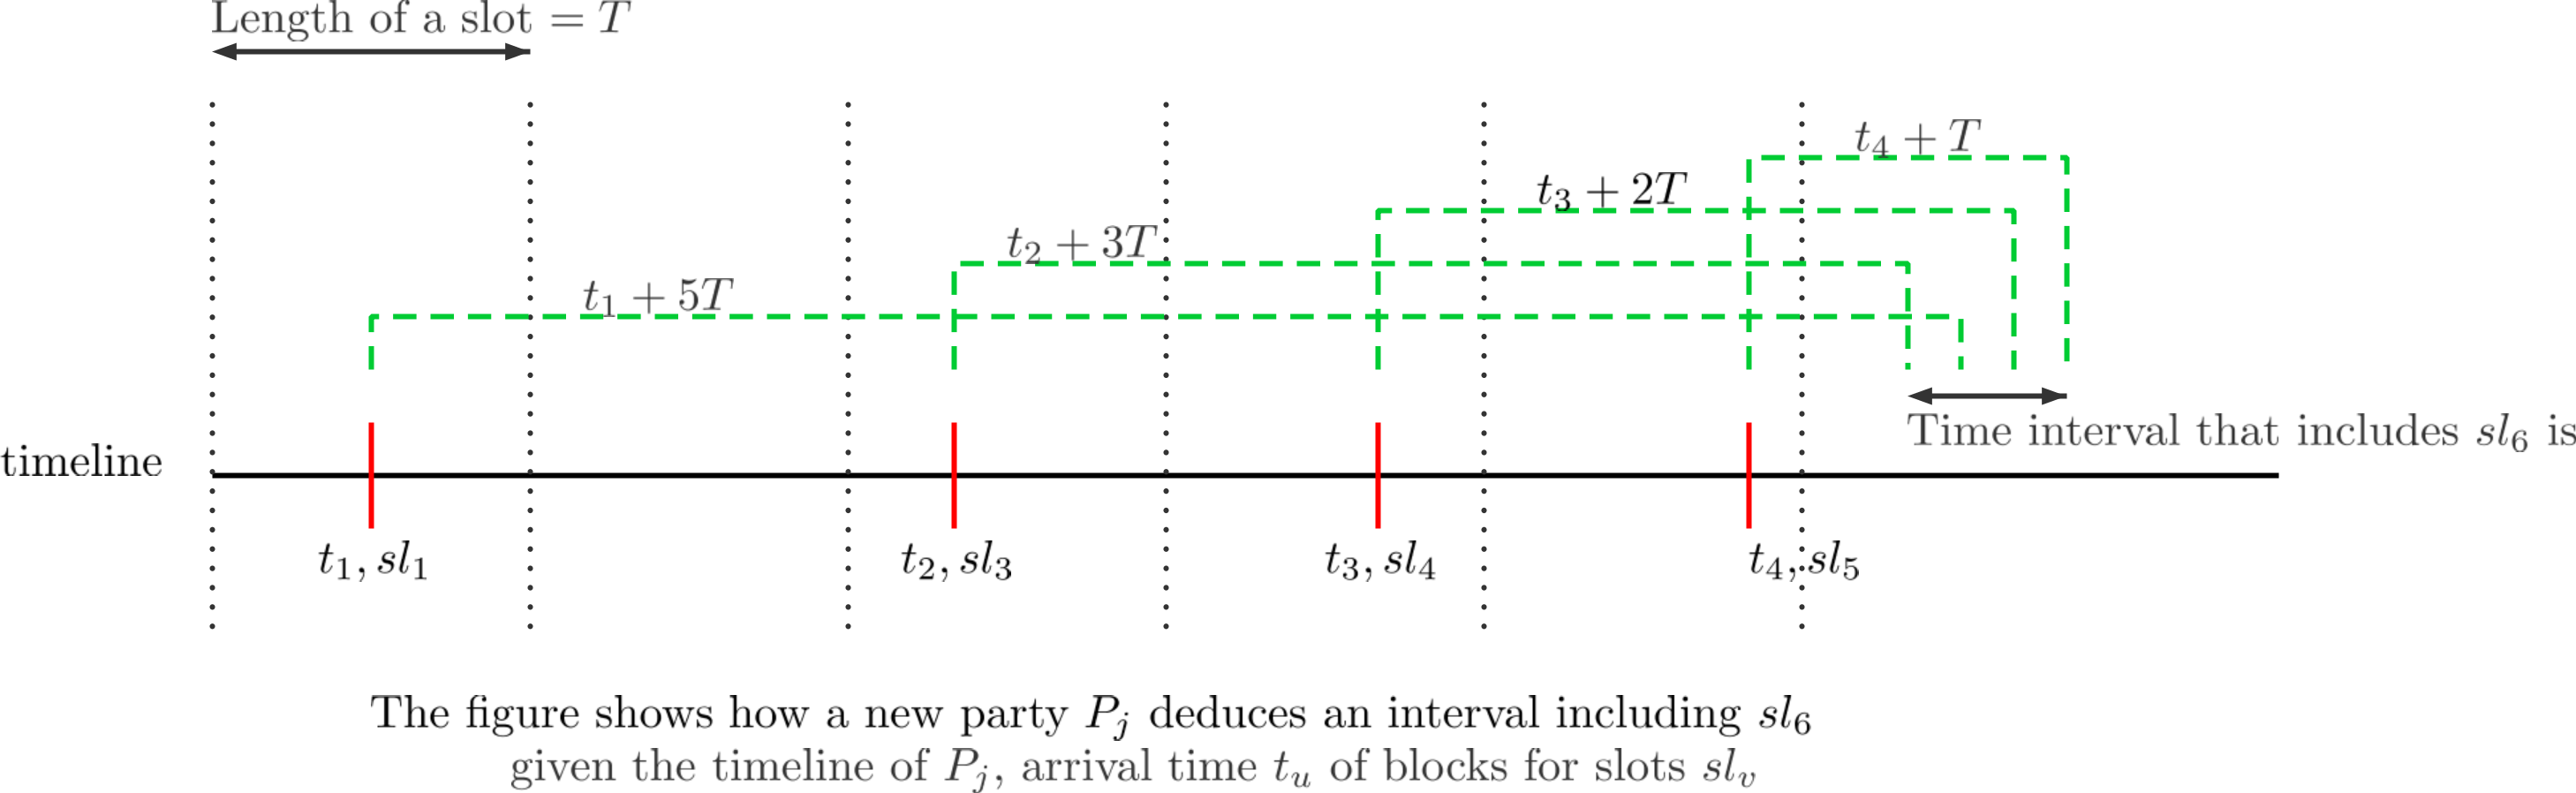
\includegraphics[width=1.\textwidth]{images/relative.png}
	\caption{An example execution of the relative time protocol by a validator who wants to learn $ \slot_{6} $.}
	\label{fig:relativetime}
\end{figure}
